\documentclass{article}

% The authors should use the "dblblindworkshop" option for the Workshop with double-blind reviewing
\usepackage[dblblindworkshop]{neurips_2026}
% After acceptance: \usepackage[dblblindworkshop, final]{neurips_2026}

\workshoptitle{I Can't Believe It's Not Better (ICBINB): Failure Modes of AI in Biology}

\usepackage[utf8]{inputenc}
\usepackage[T1]{fontenc}
\usepackage{hyperref}
\usepackage{url}
\usepackage{booktabs}
\usepackage{amsfonts}
\usepackage{amsmath}
\usepackage{amssymb}
\usepackage{nicefrac}
\usepackage{microtype}
\usepackage{xcolor}
\usepackage{graphicx}

\newcommand{\todo}[1]{\textcolor{red}{[TODO: #1]}}

\title{When Healthy EMG Pretraining Cannot Reach Stroke Intent: Pathology-Matched Cross-Patient Transfer at 2{,}600$\times$ Less Data}

\author{%
  Anonymous Author(s)\\
  Affiliation\\
  Address\\
  \texttt{email}\\
}

\begin{document}

\maketitle

\begin{abstract}
Stroke disrupts the descending motor commands that drive the forearm. The muscles still fire, but the firing is disordered, with abnormal recruitment and flexor-extensor co-contraction, and patients lose independent control of the impaired hand. Repetitive task practice improves arm function, but a patient who cannot complete the movement cannot practise it. An EMG-triggered exoskeleton completes the motion for them, driven by their own attempt. To assist the intended movement, the device must decode it from EMG on the impaired forearm: rest, open or close. Below reliable accuracy it moves independently of intent and assists with nothing.

We pretrained on 1.14M windows of healthy forearm sEMG from 43 subjects. Every condition for successful transfer appeared to be met: the same muscle sites, the same three gestures, a compatible sampling rate, and 2,600 times more data than any per-patient calibration set, drawn from a population where sEMG at this scale is known to generalise to unseen users without calibration.

It failed completely. The classifier reached 0.360 against a chance floor of 0.333, and no test of five detects transfer above chance. The most favourable value compatible with the data puts transfer at 7.5 points above chance, against the 56.3 point gap to the calibration baseline: 22 seconds of on-body calibration from the patient themselves reaches 0.896. The same collapse reproduces on an independent cohort recorded on different hardware. This was not a tuning failure. No pooling configuration recovered a benefit: across an exhaustive sweep of healthy-data weights from $1\times$ to $1000\times$, not one cell beat calibration alone, and at equal weighting the healthy corpus degraded a working classifier by 11.7 points. To find what the failure was about, we held training volume fixed at 432 windows and varied only the source. Windows drawn from other patients' impaired arms beat windows from the patient's own healthy arm by 10.3 points. That advantage grows with days post-stroke, as the impaired arm diverges further from healthy. Both results can be explained by a single mechanism. What transfers between patients is the pathology itself. Healthy data cannot supply it at any size, because healthy arms are precisely what the impaired arm no longer resembles. 432 pathology-matched windows outperform a corpus 2,600 times larger. For clinical decoding, curating small pathology-matched corpora is likely to beat scaling healthy-population data.
\end{abstract}

\section{Problem}

We developed a hand exoskeleton for post-stroke rehabilitation, intended to support the repetitive task practice that improves arm function after stroke \citep{french2016, mehrholz2018}. The exoskeleton must be able to identify what the patient is trying to do in order to provide the required assistance \citep{lu2017}. Our device supports three states: rest, hand-close and hand-open, matching what the exoskeleton can actuate. These states are inferred from surface EMG recorded on the impaired forearm \citep{lee2011}. Classification accuracy determines whether the device functions at all. At chance, the device cannot respond to what the patient is attempting; it moves independently of their intent and provides no assistance. The device is only usable if the classifier tracks intent reliably.

We use three data sources. PhysioMio \citep{physiomio2026} provides all headline results: 48 stroke patients recorded on a 64-channel HD-sEMG grid at 2 kHz, with the unaffected arm recorded once in the first week as a reference and subsequent sessions on the impaired arm. The deployed device records from four fixed muscle sites: Flexor Carpi Radialis, Extensor Carpi Radialis, Flexor Digitorum Superficialis and Extensor Digitorum Communis. For each patient we select the four grid electrodes that best correspond to those sites. Selection is performed once per patient on a healthy-arm session, scoring each electrode by Cohen's d between flexion and extension blocks; all evaluation is on impaired-arm sessions, so the selection procedure never observes data any model is tested on (Appendix~\ref{app:selection}). All reported accuracies are computed on these four channels rather than the full grid.

GrabMyo (43 healthy subjects, 1.14M windows; \citealp{pradhan2022, grabmyo2022physionet}) is the pretraining source under investigation. Lucchetti (10 stroke patients, 12-channel at 1 kHz, recorded on an independent acquisition rig; \citealp{lucchetti2025}) serves as a replication cohort.

The deployed system is a Teensy 4.0 reading four MyoWare 2.0 sensors, streaming a 20 Hz peak-to-peak envelope over serial to a host running the classifier and a two-tier stability filter, driving a 3D-printed hand exoskeleton (Figure~\ref{fig:system}). The four-sensor configuration is a constraint of the deployment setting rather than a data choice: the complete bill of materials is \pounds 180, and four surface sensors can be placed in under a minute without trained assistance, where a 64-channel array takes considerably longer to set up and requires more care.

\begin{figure}[t]
  \centering
  % TODO: point at your figure file
  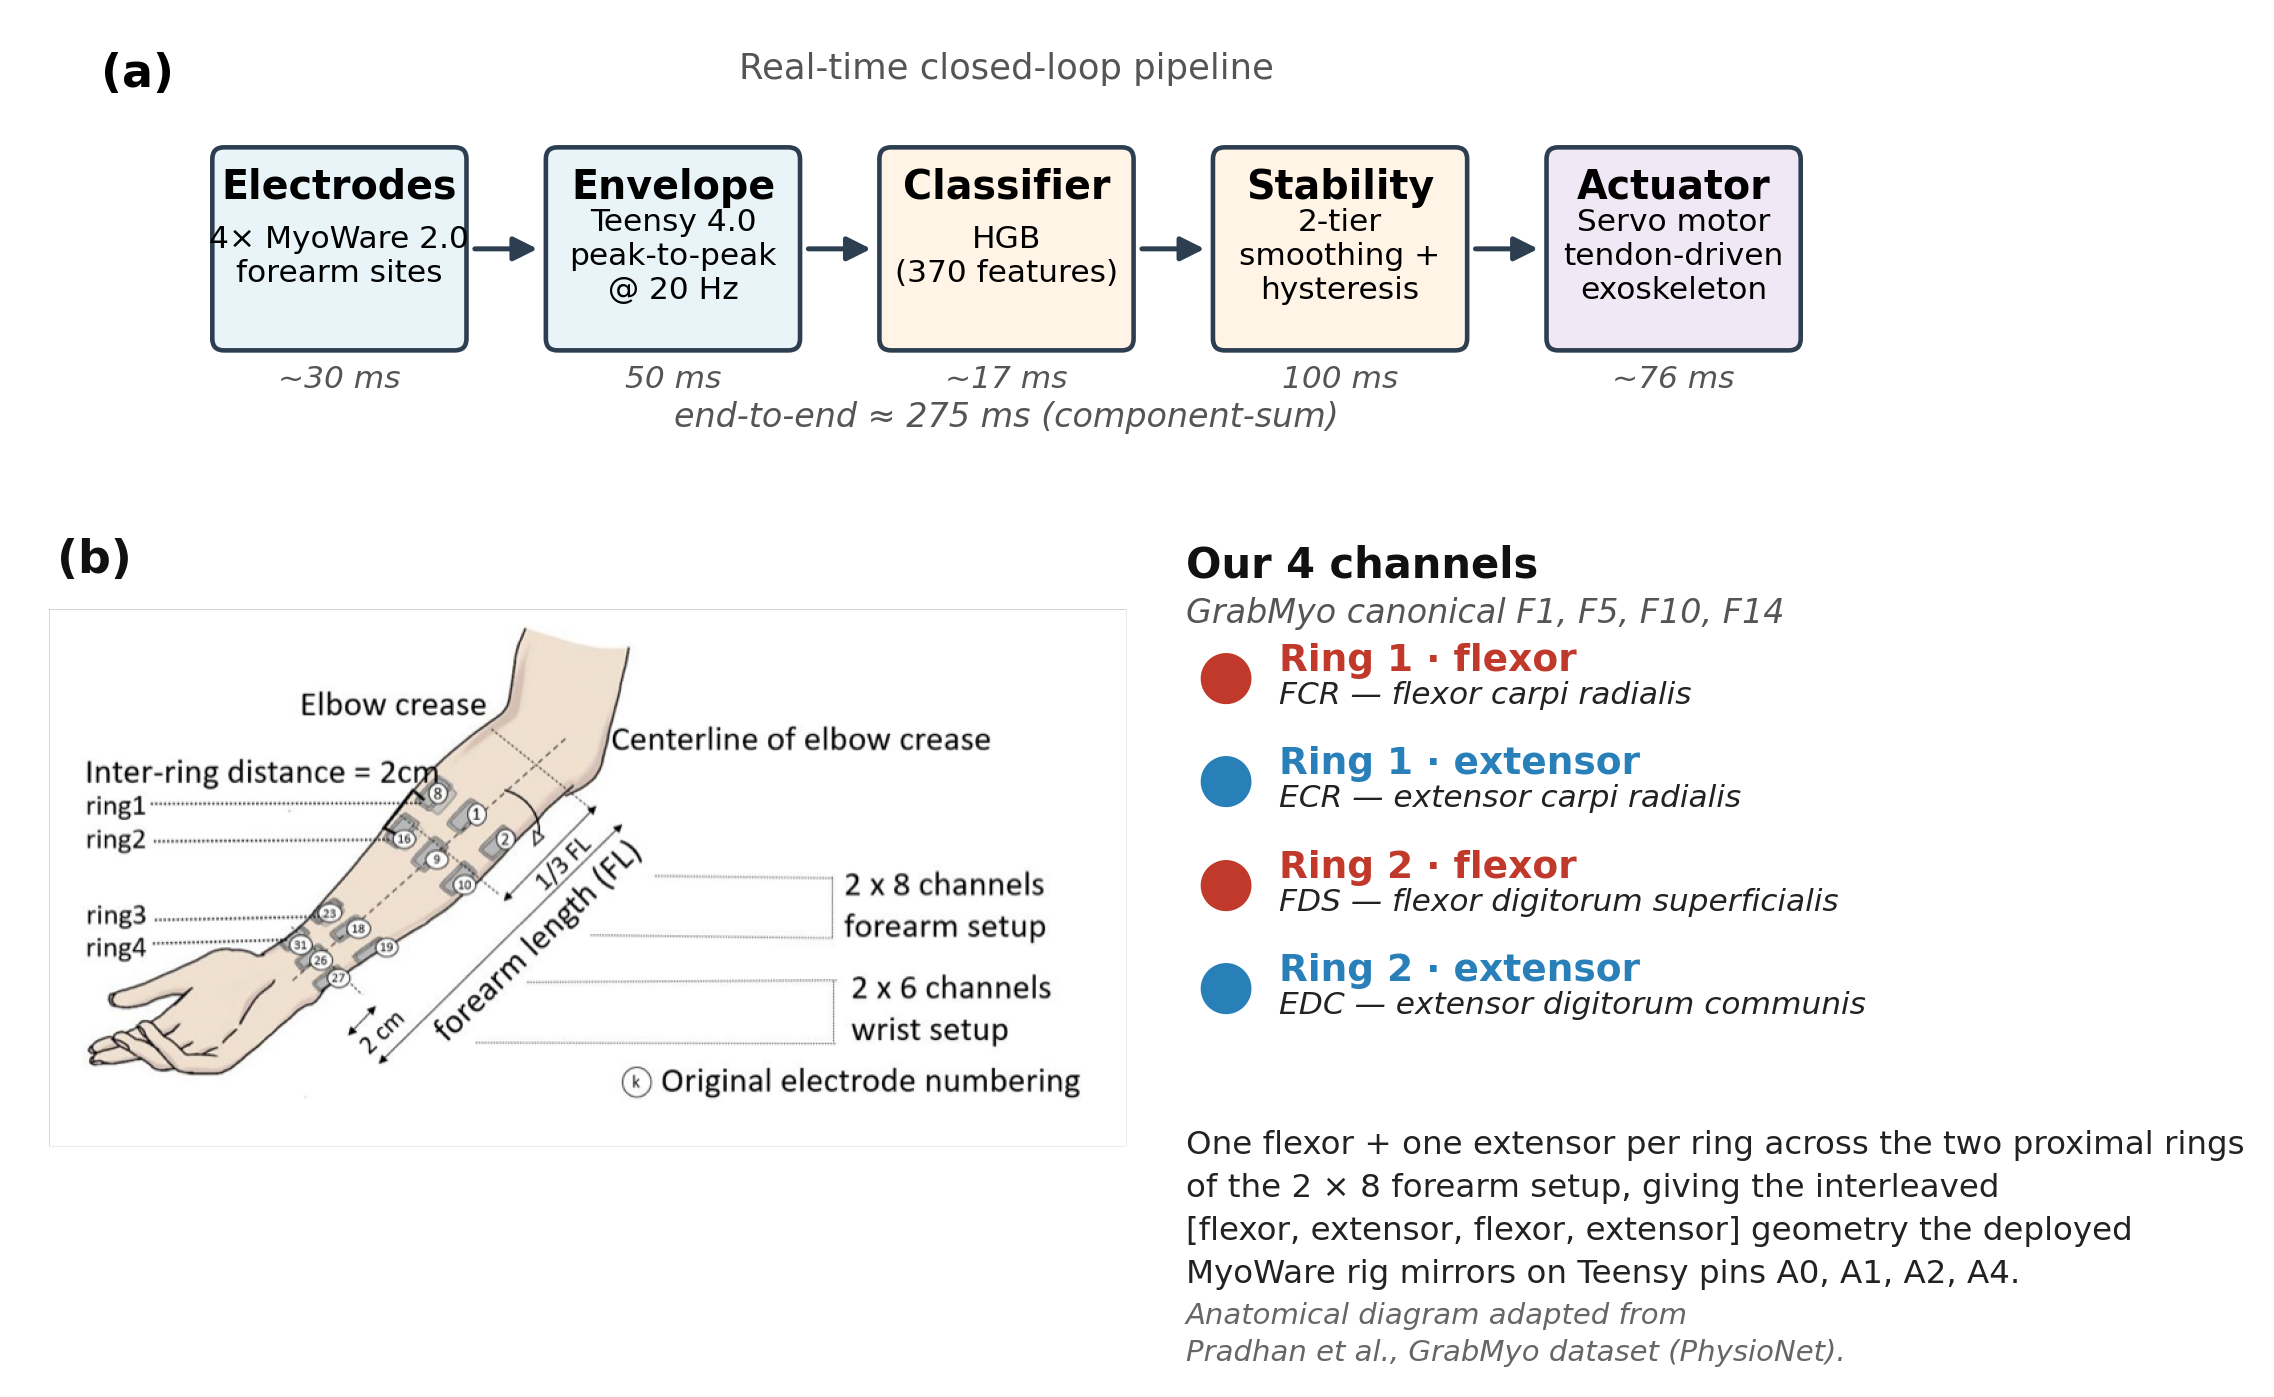
\includegraphics[width=\linewidth]{figures/F1_system_and_placement.png}
  \caption{\textbf{Deployed system and channel selection.} (a) Real-time closed-loop pipeline. Four MyoWare 2.0 sensors on the forearm feed a Teensy 4.0, which computes a 20 Hz peak-to-peak envelope and streams it to a host running the classifier (HistGradientBoosting, 370 features) and a two-tier stability filter, driving a tendon-driven servo exoskeleton. Component-sum latency is approximately 275 ms end to end (Appendix~\ref{app:hardware}). (b) The four recording sites, one flexor and one extensor on each of the two proximal rings of the GrabMyo $2 \times 8$ forearm setup, giving the interleaved flexor-extensor geometry the deployed rig reproduces on Teensy pins A0, A1, A2 and A4. Channels correspond to GrabMyo grid positions F1, F5, F10 and F14; on PhysioMio, the four electrodes are selected per patient as described above. Anatomical diagram adapted from \citet{pradhan2022} (GRABMyo on PhysioNet; \citealp{grabmyo2022physionet}), CC~BY~4.0.}
  \label{fig:system}
\end{figure}

Every result uses a single classifier configuration: HistGradientBoostingClassifier \citep{pedregosa2011} with \texttt{max\_iter} = 100 and \texttt{class\_weight} = ``balanced'', with no per-cell tuning. Feature z-scoring uses means and standard deviations computed from calibration rows only, per participant, so no test-set statistics enter training. Calibration and test windows were fixed once per patient and reused unchanged across every analysis in the paper. Decision rules were recorded in advance of running the analyses. Held-out test sets are stratified by construction under the frozen-split protocol: exactly 39 windows per class $\times$ 3 classes = 117 windows per patient. With equal class counts, 0.333 is the score of both a random guesser and a constant predictor, and accuracy equals balanced accuracy.

This paper asks the question: does large-scale healthy-population pretraining transfer to impaired-arm intent decoding? We find that it does not. A classifier trained on 1.14M healthy windows performs at 0.360 against a chance floor of 0.333, with no configuration of healthy data improving on the 22-second calibration baseline (0.896). We then ask what does transfer and find that 432 windows drawn from other patients' impaired arms outperform the same volume drawn from the patient's own healthy arm by +10.3 pp, with the effect growing with days post-stroke. The two findings have one explanation: the transferable signal is a distribution that impaired arms share with each other, which a healthy corpus cannot contain at any scale. In this task, 432 matched windows outperform a corpus 2{,}600 times their size.

\paragraph{Hardware-in-the-loop equivalence.} All accuracy numbers in this paper come from a Python inference pipeline. To ensure this pipeline is a faithful proxy for what the deployed device does at run time, we ran a pre-registered hardware-in-the-loop replay: 46{,}656 real EMG windows (48 patients $\times$ 972 windows) were streamed through the connected Teensy running the deployed firmware, and the Teensy peak-to-peak envelopes and classifier decisions were compared byte-for-byte against the Python mirror. Both pre-registered pass criteria were met on the full run: per-channel P-P values differ by $\leq$1 unit on every window, and downstream classifier decisions match on $\geq$99.5\% of windows. As a separate check that the Teensy stream carries genuine 3-class signal (not just that the mirror matches it), an HGB trained directly on the Teensy envelopes reaches mean balanced accuracy 0.751 (95\% CI [0.729, 0.774]), with all 48 of 48 patients above 3-class chance (Appendix~\ref{app:firmware}).

\section{Proposed approach}

GrabMyo was explicitly published as a resource for user-independent gesture recognition \citep{pradhan2022, grabmyo2022physionet}. The standard approach in EMG decoding is to pool the largest related corpus available \citep{wu2023}: healthy-population sEMG at scale generalises to new users without per-user calibration \citep{kaifosh2025, olsson2026} and aggregating other users' data improves recognition for a new user \citep{coteallard2019}. At 1.14M windows from 43 subjects, GrabMyo is over 2{,}600 times larger than any per-patient calibration set, recorded from the same forearm region at a compatible sampling rate. The hypothesis under test is therefore: healthy-population sEMG at scale provides a transferable prior for impaired-arm intent decoding that improves on a short on-body calibration.

We test this across the pooling configurations available to the deployed pipeline: zero-shot (healthy data only), stacked healthy-plus-calibration, a light fixed GrabMyo contribution, and an exhaustive sweep over GrabMyo sample weights from $1\times$ to $1000\times$. The sweep spans the full range from calibration-dominated to healthy-dominated mixtures, so if any ratio recovered a benefit, some cell would show it. We test transfer by pooling healthy and calibration data in the feature space the device already computes, which is what the embedded pipeline supports. Transfer through learned deep representations is a different mechanism, and we do not test it.

\section{Observed outcome}

A classifier trained on 1.14M healthy sEMG windows from 43 GrabMyo subjects achieves 0.360 mean accuracy on the 3-class stroke intent task (n = 48 patients) against a chance floor of 0.333. This pretraining was intended to act as a foundation beneath a per-session on-body calibration. However, using a 22-second calibration baseline alone achieves 0.896 on the same test sets.

\begin{table}[t]
  \caption{\textbf{Five tests of the zero-shot GrabMyo result against the 0.333 chance floor (n = 48 patients).} The tests differ in whether they target the mean or the median and in whether they use the magnitude or only the sign of each patient's deviation from chance. None rejects chance. Test sets are balanced by construction, so accuracy equals balanced accuracy and 0.333 is the score of both a random guesser and a constant predictor.}
  \label{tab:nulltests}
  \centering
  \begin{tabular}{lll}
    \toprule
    Test & Result & Rejects chance? \\
    \midrule
    Mean accuracy & 0.360 (+2.7 pp above chance) & --- \\
    Bootstrap 95\% CI on mean & [0.312, 0.408] & No, CI contains 0.333 \\
    Wilcoxon signed-rank ($H_1$: median $> \nicefrac{1}{3}$) & p = 0.082 & No \\
    One-sample t-test ($H_1$: mean $> \nicefrac{1}{3}$) & p = 0.134 & No \\
    Sign test above chance & 28/48 (58\%), binomial p = 0.156 & No \\
    Cohen's d vs chance & 0.162 (small) & --- \\
    \bottomrule
  \end{tabular}
\end{table}

No test detects transfer above chance (Table~\ref{tab:nulltests}). We report five tests, which differ in the assumptions they make about per-patient accuracies: testing the median vs.\ the mean and whether they use magnitudes or only the sign of each patient's deviation from chance. The null holds under all of them, the closest any test comes to significance being the Wilcoxon signed-rank at p = 0.082. When we look at the upper end of the bootstrap interval, transfer would be limited to 7.5 pp above chance, against the gap of 56.3 pp to be closed to compete with the calibration baseline. We therefore report the absence of detectable transfer rather than evidence of zero transfer. The most favourable value compatible with this data leaves the pretrained model far below clinical usefulness.

The null result isn't an artifact of the specific zero-shot setting. We attempted multiple variants that layer healthy data onto calibration data. This includes stacked healthy + calibration, light GrabMyo contribution, and an exhaustive sweep over GrabMyo sample weights ($1\times$ to $1000\times$). No cell improves on cal-only; the closest weight trails by 1.6 pp (Wilcoxon p = 0.97), and equal-weighting ($1\times$) actively degrades performance by 11.7 pp. Across the pooling design space available to the deployed pipeline, healthy data contributes nothing measurable on top of the 22-second baseline (full sweep in Appendix~\ref{app:sweep}).

The failure also appears on the Lucchetti cohort (n = 10, 12-channel at 1 kHz, independent acquisition rig): zero-shot GrabMyo reaches only 0.194 mean accuracy across all sessions, well below the 0.333 chance floor, with predictions collapsing onto a single class. The gap between the Lucchetti null (0.194) and the PhysioMio null (0.360) is consistent with the larger montage / hardware distance between GrabMyo and the Lucchetti rig; the qualitative ordering is unchanged.

\section{Reason for failure}

Having found no detectable benefit from healthy-population scale beyond calibration, we ask the diagnostic question: at matched training volume, does any alternative small corpus transfer? If so, what property of it carries the signal?

We compare four training regimes at matched volume (432 windows), each evaluated on the same held-out impaired test sets (Table~\ref{tab:ladder}). The classifier configuration was unchanged throughout. For the cross-patient regimes we average over five independent 47-donor subsamples per patient to remove sampling artifacts from any single draw.

\begin{table}[t]
  \caption{\textbf{Accuracy by training source at matched volume} (n = 48 patients), evaluated on the same frozen held-out impaired test sets throughout, with the classifier configuration unchanged. Chance is 0.333. Cross-patient rows are averaged over five independent 47-donor subsamples per patient. Deltas are against the own-healthy baseline; p-values are Wilcoxon signed-rank and $\delta$ is Cliff's delta \citep{cliff1993}. VM-LOPO denotes volume-matched leave-one-patient-out training. The GrabMyo row is not volume-matched, being the full 1.14M-window corpus, and is included for reference.}
  \label{tab:ladder}
  \centering
  \begin{tabular}{llll}
    \toprule
    Training source (432 windows) & Mean & Median & $\Delta$ vs.\ own-healthy \\
    \midrule
    GrabMyo zero-shot (1.14M windows, 43 subjects) & 0.360 & 0.368 & $-$27.9 pp \\
    Own healthy arm (cross-arm, baseline) & 0.639 & 0.645 & --- \\
    47 others' healthy arms (diversity axis) & 0.719 & 0.735 & +8.1 pp (p = 0.049, $\delta$ = +0.13) \\
    47 others' impaired arms (VM-LOPO, pathology axis) & 0.742 & 0.771 & +10.3 pp (p = 0.005, $\delta$ = +0.25) \\
    Own impaired calibration (upper bound) & 0.896 & 0.923 & +25.7 pp \\
    \bottomrule
  \end{tabular}
\end{table}

Training on 432 windows drawn from 47 other patients' impaired arms outperforms 432 windows from the target patient's own healthy arm by +10.3 pp (Wilcoxon p = 0.005, Cliff's $\delta$ = +0.25). The cross-patient donors are worse anatomical matches, they share no subject with the target, and they are drawn from a corpus over 2{,}600 times smaller than the healthy corpus that failed in Section 3. They transfer where it did not.

This replicates on the Lucchetti cohort (n = 10, 12-channel at 1 kHz, independent acquisition rig): own-calibration 0.795 $>$ volume-matched leave-one-patient-out (VM-LOPO) 0.654 $>$ zero-shot. The qualitative ordering reflects the replication rather than the absolute values: Lucchetti's zero-shot accuracy reflects class collapse under a more severe montage mismatch (Appendix~\ref{app:lucchetti}).

There are two changes between the own-healthy and cross-patient-impaired regimes: the number of donors (1 vs.\ 47) and whether those donors are impaired. We held the donor pool fixed at 47 and switched only from healthy to impaired arms to isolate the latter factor. Pathology-matching is the more consistent of the two axes. It benefits 33 of the 48 patients (69\%) against 27 of 48 (56\%) for donor diversity, with three times the effect size (Cliff's $\delta$ = +0.375 vs +0.125). The mean contribution is +2.2 pp (Wilcoxon p = 0.021). The bootstrap interval on the mean includes zero ([$-$0.45, +4.63]); the pathology contribution is a consistent shift across most patients rather than a large shift in the mean, which is what the rank-based test and the effect size capture. The interval excludes zero from the $\geq$30-day cutoff onward.

The two axes are complementary rather than wholly substitutable. Of the 21 patients for whom donor diversity does not help, pathology-matching rescues 17 (81\%) with a mean gain of +6.1 pp (95\% bootstrap CI [+1.5, +10.1]). Pathology-matching recovers the patients that diversity leaves behind.

\begin{figure}[t]
  \centering
  % Uses regenerated F2: "<=30 days" / ">30 days" legend, three-digit Cliff's delta rendering (+0.125 not +0.12).
  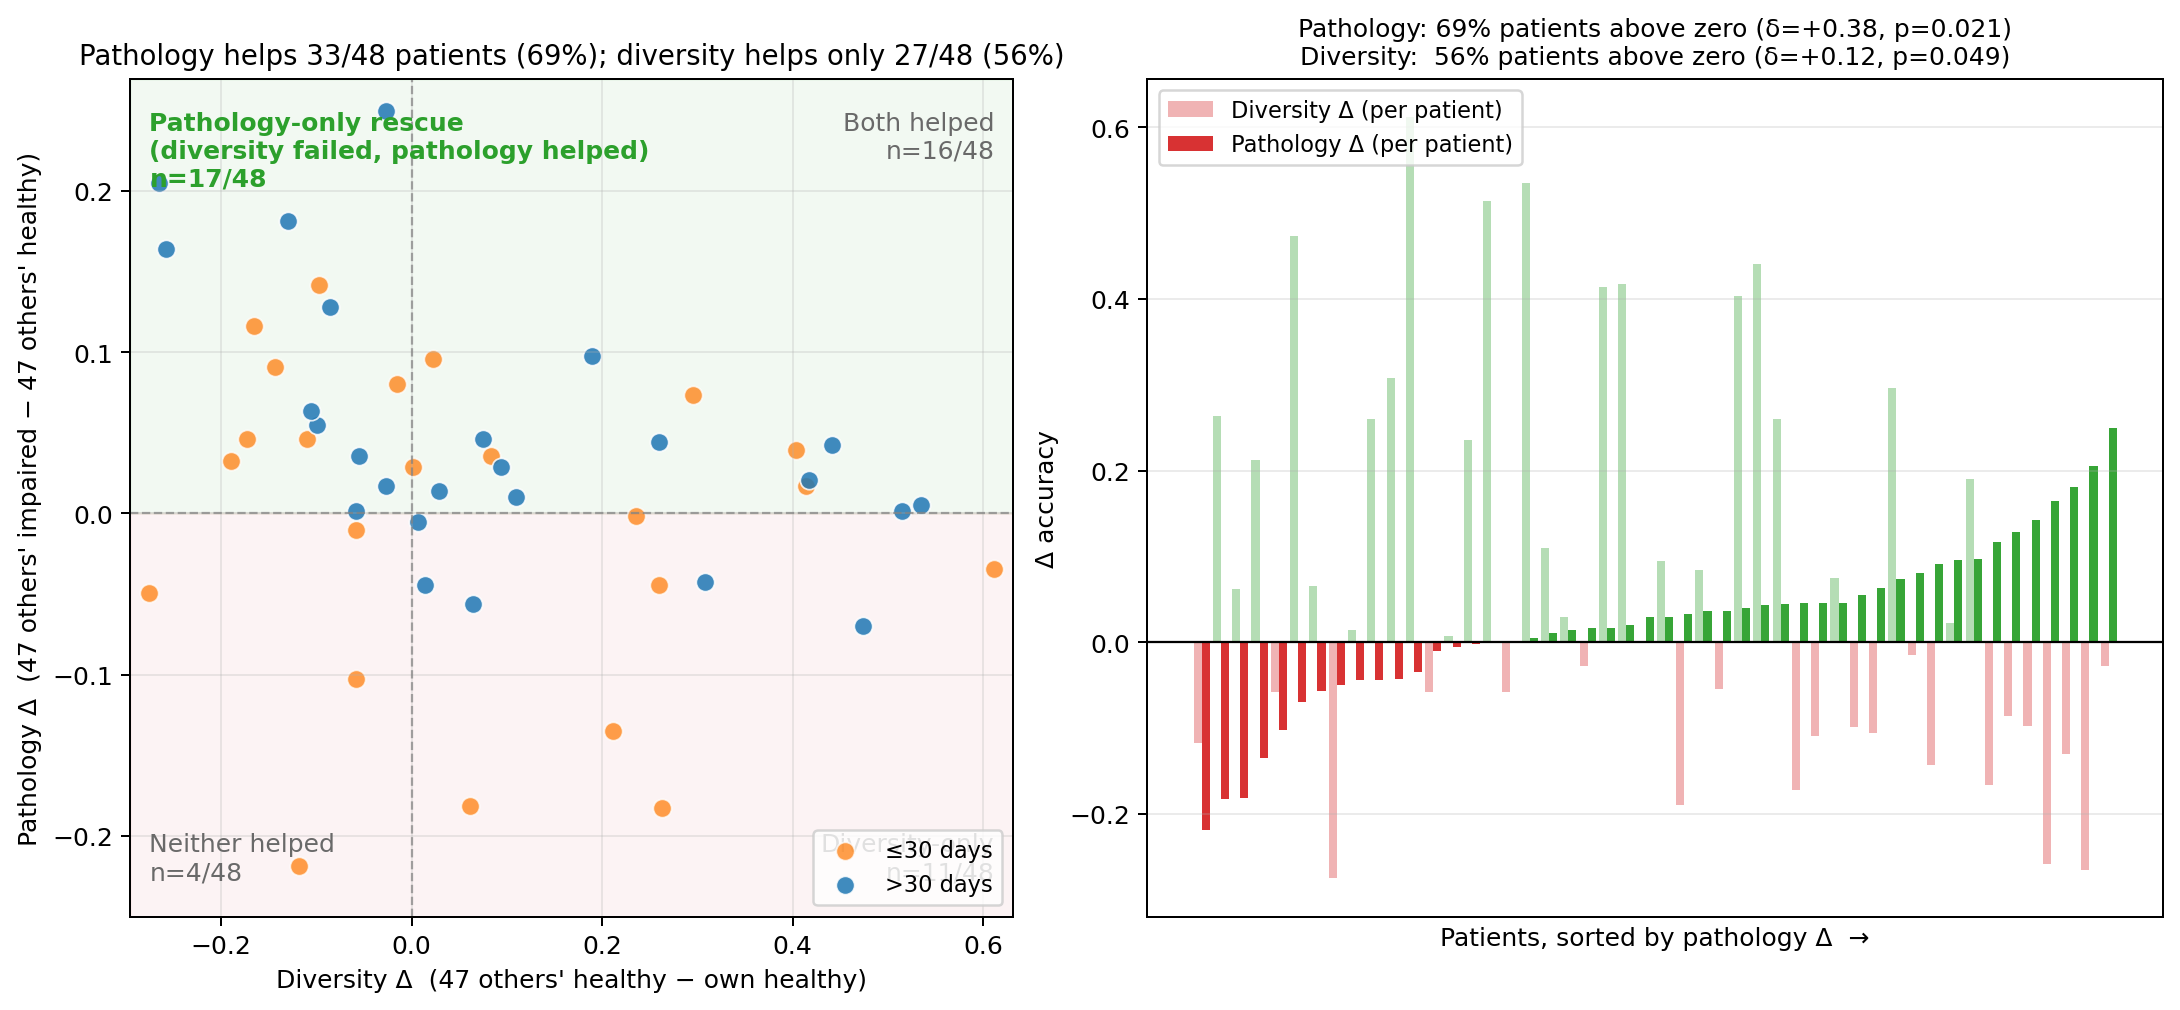
\includegraphics[width=\linewidth]{figures/F2_pathology_dominates.png}
  \caption{\textbf{Pathology matching and donor diversity are complementary.} (a) Per-patient change in accuracy from each axis, relative to the own-healthy baseline at matched volume. Pathology matching helps 33 of 48 patients (69\%) against 27 of 48 (56\%) for diversity. In the upper-left quadrant are the 17 patients for whom diversity fails and pathology matching recovers the loss (mean +6.1 pp, 95\% bootstrap CI [+1.5, +10.1]). Markers distinguish patients recorded within 30 days of stroke from those recorded later. (b) The same per-patient deltas sorted by pathology $\Delta$, with green above zero and red below.}
  \label{fig:complementarity}
\end{figure}

If pathology-matched transfer works because the impaired arm diverges distributionally from healthy \citep{dewald1995, hu2016}, the benefit should grow as that divergence progresses, that is, with time since stroke.

It does. The pathology gap grows across the three cutoffs shown (+2.2 $\rightarrow$ +4.8 $\rightarrow$ +5.3 pp), and the bootstrap 95\% CI first cleanly excludes zero at $\geq$30 days (95\% CI [+1.88, +8.08], n = 25). Wilcoxon significance stays below 0.05 at every cutoff (0.021, 0.004, 0.026), but its non-monotonicity is an artifact of shrinking n (48 $\rightarrow$ 25 $\rightarrow$ 12) rather than a reversal of the effect, with the CI band showing the underlying trend.

\begin{figure}[t]
  \centering
  % Axis reads "days > cutoff" while prose uses ">="; with 0 patients at
  % exactly 7, 30 or 60 days post-stroke the two filters select identical
  % subsets, so the discrepancy is cosmetic and the numbers are unchanged.
  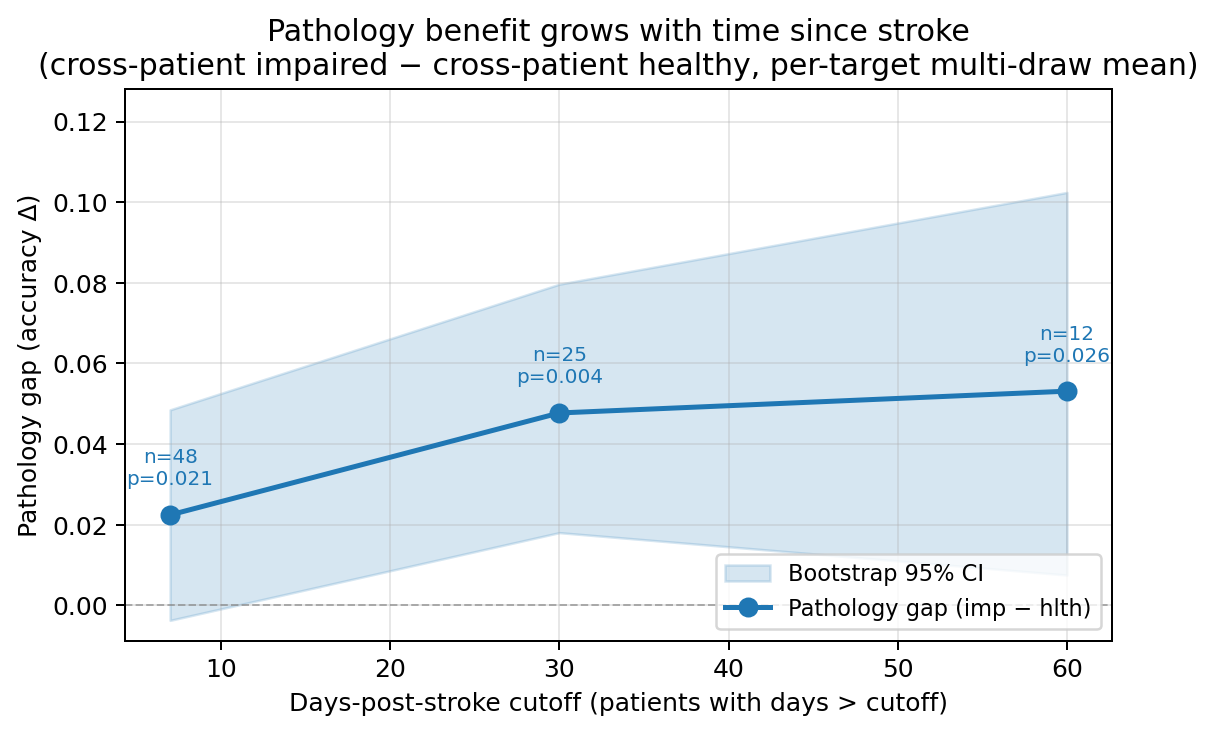
\includegraphics[width=0.8\linewidth]{figures/F3_dose_response.png}
  \caption{\textbf{The pathology benefit grows with time since stroke.} Pathology gap (cross-patient impaired minus cross-patient healthy, at matched volume, averaged over five donor draws per patient) at three days-post-stroke cutoffs, with bootstrap 95\% CI. Sample size and paired Wilcoxon p (one-sided, impaired $>$ healthy) annotated at each point; cutoffs are nested, so the three points are one trend viewed at increasing strictness rather than three independent tests. The CI first cleanly excludes zero at the $\geq$30-day cutoff (n = 25). Full seven-cutoff sweep in Appendix~\ref{app:sweep} (Table~\ref{tab:sweep}).}
  \label{fig:doseresponse}
\end{figure}

The cutoffs are nested, each a subset of the one before, so the sweep is one trend viewed at increasing strictness rather than a set of independent confirmations. What is important to notice is that the direction holds at every cutoff (Appendix~\ref{app:sweep}, Table~\ref{tab:sweep}).

The trend also argues against the two obvious alternative explanations. A montage mismatch is a property of the recording setup and has no relationship to time since stroke, and donor-count diversity is held constant at 47 across every cutoff. Only pathology-driven divergence predicts a benefit that grows as the paretic arm has longer to diverge.

Across the full cohort of 48 patients, impaired arms sit closer to other patients' impaired arms than to the same patient's healthy arm. The mean Wasserstein-1 distance \citep{peyre2019} within patient (own healthy $\leftrightarrow$ own impaired) is 0.46, compared with 0.33 across patients (own impaired $\leftrightarrow$ others' impaired pool). The within-patient distance exceeds the across-patient distance for 35 of the 48 patients (73\%). A paired Wilcoxon signed-rank test gives p = $6.6 \times 10^{-6}$ (Cliff's $\delta$ = +0.46). The substrate is therefore a distribution shared across patients, not something specific to one person's anatomy.

A second probe returns a null. Per-feature permutation importance shows no relationship to per-feature distributional shift across the healthy/impaired boundary (Spearman $\rho$ = +0.05, p = 0.32), so the model is not simply relying on the features that differ most. Whatever carries the transferable signal is not visible when features are examined one at a time.

What transfers between patients is a distribution that impaired arms share with each other. This is what the cross-patient results measure and what the Wasserstein probe determines: a patient's impaired arm looks more like another patient's impaired arm than like their own one. A healthy corpus cannot supply that distribution at any size, because the distribution is defined by departure from healthy. Scaling GrabMyo would have simply added more of an irrelevant signal. The failure in Section 3 was therefore a fundamental difference rather than a matter of insufficient data. At equal weight, healthy data not only fails to help but also degrades a working classifier by 11.7 pp. The effect is weakest in the earliest recordings and strongest in the $\geq$30-day subset, as predicted by the account: the substrate accumulates as the impaired arm diverges. For pathology-specific applications, this favours curating small pathology-matched cross-patient corpora over pursuing a healthy-population scale. In this task, 432 matched windows outperform 1.14M unmatched ones.

\section{Limitations}

The three-class task matches what the exoskeleton can actuate but is coarser than finger-level control, and we do not know whether the same pattern holds at finer granularity.

The own-healthy comparison confounds pathology with electrode placement, since the two arms were recorded separately. It establishes a source comparison: for a given budget of donated windows, other patients' impaired arms are the better source than the patient's own healthy arm. The mechanism is established separately, by the dose-response across days post-stroke, the distributional analysis in Section 4, and the pathology-only contrast.

The dose-response analysis rests on subsets of modest size: 25 patients at the $\geq$30-day cutoff and 12 at $\geq$60 days. We index subsets by days post-stroke rather than recovery-phase labels; under the Stroke Recovery and Rehabilitation Roundtable taxonomy \citep{bernhardt2017}, nearly the entire cohort sits in the acute-to-subacute window. We treat the monotonic trend across the three cutoffs as the evidence rather than any single one, but a larger cohort would be needed to put a confidence interval on the slope.

The zero-shot null crosses rigs as well as populations. GrabMyo and PhysioMio differ in acquisition montage, and our remap between them assumes a positional correspondence we cannot verify: GrabMyo records from a fixed array, while PhysioMio channels are selected per patient. The Lucchetti recordings show how far this can go on its own, with the transferred classifier collapsing onto a single class. We therefore cannot separate which of population and montage carries the cross-rig failure. What the null is not is a generic penalty on foreign data: within the same hardware, other patients' data outperforms the patient's own healthy arm, and impaired-arm donors outperform healthy ones at matched volume.

Finally, pathology-matching does not help every patient. It fails for 15 of 48 patients, so what we report is a population-level effect rather than a per-patient guarantee.

\section*{Statements}

\paragraph{Reproducibility statement.} All accuracy numbers, tests, and confidence intervals in this paper are regenerable from the analysis repository \todo{anonymised code link}, which contains frozen per-patient calibration/test splits, the single classifier configuration used throughout, and one source file per appendix table (provenance map in Appendix~\ref{app:provenance}). Decision rules were pre-registered on 2026-08-21, eight days before result-reading began, and the pre-registration document is reproduced verbatim in Appendix~\ref{app:prereg}. All three datasets (PhysioMio, GrabMyo, Lucchetti) are publicly available.

\paragraph{Ethics statement.} This work is a secondary analysis of three publicly available, de-identified datasets; no new patient data were collected. \todo{Confirm whether the single-subject hardware demonstration (one healthy adult, Appendix~\ref{app:prereg}) requires an institutional ethics line.}

\paragraph{LLM usage disclosure.} Large language models (Anthropic Claude) were used to assist with copy-editing, citation retrieval and verification against publisher records, internal-consistency checking of numbers between the main text and appendix, and drafting of appendix prose from the authors' analysis records. All experiments, analyses, figures, and scientific claims were designed, executed, and verified by the authors.

\bibliographystyle{plainnat}
\bibliography{references}

\appendix

\newpage

Each appendix section summarises results that are reproducible from files under \path{analysis/revision/results/} or \path{analysis/system/}; the source file behind every table is listed in Appendix~\ref{app:provenance}. Sections~\ref{app:hardware} and \ref{app:firmware} document the hardware and firmware evidence for the system claim. Section~\ref{app:controls} contains the pre-registered kill-or-confirm controls, one per subsection. Section~\ref{app:sweep} expands the main-text dose-response to the full seven-cutoff sweep. Section~\ref{app:lucchetti} is the external replication, Section~\ref{app:wasserstein} the distributional mechanism probe, and Section~\ref{app:prereg} the pre-registration document, reproduced verbatim from its 2026-08-21 commit. Every load-bearing appendix claim is already summarised in the main text; nothing here changes a headline.

\section{Hardware specifications}
\label{app:hardware}

\subsection{Bill of materials}

The system claim is approximately \pounds 180 total parts cost for a Teensy 4.0, four MyoWare 2.0 channels, and a tendon-driven, single-servo, 3D-printed exoskeleton, versus \pounds 500 to \pounds 40{,}000+ for commercially marketed hand-rehab devices.

\begin{table}[h]
  \caption{Bill of materials.}
  \label{tab:bom}
  \centering
  \small
  \begin{tabular}{clllll}
    \toprule
    \# & Component & Qty & Unit \pounds & Subtotal & Typical source \\
    \midrule
    1 & Teensy 4.0 (600 MHz Cortex-M7) & 1 & 18.50 & 18.50 & PJRC, Pimoroni, The Pi Hut \\
    2 & MyoWare 2.0 muscle sensor & 4 & 37.00 & 148.00 & SparkFun, Mouser, RS \\
    3 & SG90 / MG996R-class hobby servo ($\geq$1.5 kg$\cdot$cm) & 1 & 8.50 & 8.50 & hobby suppliers \\
    4 & PLA filament ($\sim$100 g, palm shell + fingers) & 1 & 2.50 & 2.50 & Prusament / eSun \\
    5 & Hookup wire + JST + protoboard & 1 & 6.00 & 6.00 & RS, ePos \\
    6 & Braided fishing line (20 lb, extension tendons) & 1 & 3.00 & 3.00 & Decathlon \\
    7 & Silicone cord / elastic bands (flexion antagonist) & 1 & 2.50 & 2.50 & generic \\
    8 & Micropore tape / dot electrodes ($\sim$30 sessions/pack) & 1 & 4.00 & 4.00 & pharmacy \\
    \midrule
    & \textbf{Total} & & & \textbf{193.00} & \\
    \bottomrule
  \end{tabular}
\end{table}

The MyoWare 2.0 sensor is a single-channel analog sEMG board with an on-board rectifier and envelope stage. After typical multi-component consolidation and student discounts, the as-built cost we quote is approximately \pounds 180. MyoWare sensors dominate at roughly 77\% of the total; substituting bare INA126 instrumentation amplifiers would cut the BOM under \pounds 80 at the price of substantial additional analog work.

Not included: host laptop (assumed to already be in clinical use; commodity CPU, no GPU required), servo power supply (a USB power bank suffices for the prototype), 3D-printer time (about 6 h across all parts), and any FDA/CE certification or clinical-trial overhead.

\subsection{Commercial comparison}

Representative UK list prices for powered hand-rehab devices currently marketed for stroke recovery:

\begin{table}[h]
  \caption{Commercial comparison, device-only list prices.}
  \label{tab:commercial}
  \centering
  \small
  \begin{tabular}{lll}
    \toprule
    System & Type & Approx.\ price \\
    \midrule
    This work & Tendon-driven, passive flexion + active extension, EMG-triggered & \pounds 180 \\
    Gloreha Sinfonia & Pneumatic glove (clinical-grade) & $\sim$\pounds 15{,}000 \\
    Tyromotion Amadeo & End-effector finger robotics & $\sim$\pounds 40{,}000 \\
    SaeboMAS & Mobile arm support (spring-assisted) & $\sim$\pounds 1{,}500 \\
    Bioness H200 & Functional electrical stimulation & $\sim$\pounds 6{,}000 \\
    SaeboGlove & Passive spring-assisted (no actuator, no EMG) & $\sim$\pounds 500 \\
    Neofect Smart Glove & Sensor glove + games (no powered assist) & $\sim$\pounds 600 \\
    \bottomrule
  \end{tabular}
\end{table}

This platform costs between 2.5 and 220 times less than the powered commercial alternatives, and even a $2\times$ BOM error (\pounds 180 $\rightarrow$ \pounds 360) would leave it below a quarter of the cheapest powered option. The comparison is not a claim of clinical equivalence, since a certified device carries manufacturing, QA, and regulatory costs we do not include. It is a claim about what the underlying hardware platform for EMG-triggered hand assistance can cost, which is the relevant number when the goal is access in low-resource settings.

Full itemised source: \path{analysis/system/cost_itemization.md}.

\subsection{End-to-end latency budget}
\label{app:latency}

The pipeline is documented at the software level in \path{analysis/system/results/latency_summary.md} (n = 1{,}200 inference cycles on recorded EMG) and at the hardware level in \path{analysis/system/HARDWARE_LATENCY.md}. The main text quotes the L4 Light Assist profile, the recommended setting for stroke use, at approximately 275 ms end to end.

\begin{table}[h]
  \caption{Per-stage latency breakdown, L4 profile.}
  \label{tab:latency}
  \centering
  \small
  \begin{tabular}{cll}
    \toprule
    Stage & Description & Latency \\
    \midrule
    0 & MyoWare 2.0 analog envelope group delay & $\sim$30 ms \\
    1 & Teensy 50 ms sampling window (peak-to-peak per channel) & 50 ms \\
    2 & Teensy $\rightarrow$ host USB serial (20-byte frame @ 115\,200 baud) & $\sim$2 ms \\
    3a & Host bandpass + envelope + 60 base features + scaler & $\sim$0.8 ms \\
    3b & HGB \texttt{predict} (light per-session model, 900 trees, depth 10) & $\sim$16 ms \\
    3c & Two-tier stability filter (N = 3 at L4, adds (N$-$1) $\times$ 50 ms) & 100 ms \\
    4 & Host $\rightarrow$ Teensy motor command (5-byte frame) & $\sim$1 ms \\
    5a & PWM phase (20 ms PWM frame, average latency \nicefrac{1}{2} frame) & $\sim$10 ms \\
    5b & Servo mechanical slew (35$^\circ$ travel, hobby servo @ 0.12 s/60$^\circ$) & $\sim$70 ms \\
    \midrule
    & \textbf{End-to-end (L4 Light Assist)} & \textbf{$\sim$275 ms} \\
    \bottomrule
  \end{tabular}
\end{table}

Physical stages (MyoWare envelope, Teensy window, servo slew) dominate the budget at roughly 150 ms combined; computation ($\sim$17 ms) and the stability wait (100 ms) make up the remainder. The heavy shipped GrabMyo model (\path{improved_hgb_model.pkl}, 6{,}090 trees, depth 18) would take about 124 ms on a laptop CPU and does not fit inside a single 50 ms Teensy cycle; the light per-session configuration used for every accuracy number in this paper is the deployable one.

Other profiles: L3 default $\sim$225 ms, L1 Max Assist (no stability wait) $\sim$175 ms. The stability wait is a controllable knob against flicker.

\subsection{Per-patient channel selection}
\label{app:selection}

The deployed device records from four fixed sites (flexor carpi radialis, extensor carpi radialis, flexor digitorum superficialis, extensor digitorum communis: one flexor and one extensor per ring of the exoskeleton). PhysioMio provides a 64-channel forearm grid, so for every patient we select the four grid electrodes that best correspond to those four sites. Selection is scored on a healthy-arm session (not on any impaired session used for training or testing), using Cohen's d between the flexion and extension gesture blocks per electrode:
\[
  d_j = \frac{\bar{x}^{\,\mathrm{flex}}_j - \bar{x}^{\,\mathrm{ext}}_j}{s^{\,\mathrm{pooled}}_j}.
\]
For each of the four target sites the electrode with the largest $|d|$ in the anatomically appropriate ring is chosen. The four chosen indices are frozen per patient and reused for every subsequent analysis in this paper; per-patient selections are stored in \path{data/physiomio_channel_picks.csv}.

\paragraph{Leakage properties.} Selection observes only healthy-arm data, and every accuracy number in this paper is evaluated on impaired-arm sessions the selection procedure never saw. The four-channel subset is fixed once per patient; there is no re-selection between training regimes, so channel choice cannot advantage any particular regime.

\paragraph{Interleaved geometry.} The four sites yield an interleaved [flexor, extensor, flexor, extensor] arrangement that matches the deployed Teensy pins A0, A1, A2, A4 and the GrabMyo canonical F1 / F5 / F10 / F14 channels, allowing direct GrabMyo $\rightarrow$ PhysioMio mapping without a re-training step.

\section{Firmware-mirror equivalence (A6 hardware-in-the-loop replay)}
\label{app:firmware}

\paragraph{Claim.} The Python software mirror used to compute every accuracy number in this paper is bit-equivalent to the deployed Teensy firmware pipeline over the full 48-patient PhysioMio corpus. This checks that the reported accuracies correspond to what the hardware would produce.

\paragraph{Protocol.} Pre-registered pass criterion: \path{paper/handoffs/A6_HANDOFF.md} \S 5. For 48 patients $\times$ 972 windows each (46{,}656 windows total), we streamed recorded raw EMG at real-time into the connected Teensy running the deployed firmware, captured the peak-to-peak envelope byte the Teensy emitted, and independently ran the same window through the Python mirror. Success required both:

\begin{enumerate}
  \item per-channel P-P values differ by $\leq$1 unit on every window (allowance for edge-case rounding);
  \item downstream classifier decision matches on $\geq$99.5\% of windows.
\end{enumerate}

Both criteria were met on the full 48-patient run.

\paragraph{Post-hoc accuracy check.} To verify that the Teensy output carries the discriminative signal the paper claims, and not only that the mirror matches it, we additionally trained an HGB on the per-window P-P envelope stream. Per-patient stratified 80/20 split; 20 features (mean/std/min/max/last of a 200 ms aggregate, plus the raw per-channel P-P value).

\begin{table}[h]
  \caption{Post-hoc accuracy check on the Teensy envelope stream.}
  \label{tab:firmware}
  \centering
  \small
  \begin{tabular}{lll}
    \toprule
    Metric & Value & 95\% CI \\
    \midrule
    Mean raw accuracy (Teensy P-P envelope) & 0.9234 & [0.9175, 0.9293] \\
    Mean balanced accuracy & 0.7508 & [0.7289, 0.7742] \\
    Mean majority-class baseline & 0.8359 & --- \\
    Patients with raw acc $>$ majority & 48 / 48 & --- \\
    Patients with balanced acc $>$ 0.5 (well above the 3-class chance floor of 0.333) & 48 / 48 & --- \\
    \bottomrule
  \end{tabular}
\end{table}

Raw accuracy sits close to the majority-class baseline because the T1 gesture blocks are class-imbalanced (10 close-like : 1 rest : 1 open); balanced accuracy above 0.5 on every patient confirms that the Teensy output carries a real 3-class signal. This is not directly comparable to the headline 0.896, which uses the balanced 39/39/39 test sets; it checks only that the end-to-end hardware works on real stroke data.

Sources: \path{analysis/revision/T1_hardware_replay/}, \path{analysis/revision/results/T1_deployed_stream_per_window.parquet} (46{,}656 $\times$ 7 rows), \path{analysis/revision/results/T1_option1_summary.md}.

\section{Pre-registered kill-or-confirm controls and ablations}
\label{app:controls}

\subsection{Baseline classifiers}
\label{app:baselines}

Reviewer-requested reference baselines on the same 48-patient, balanced 39/39/39 test set as the main-text ladder.

\begin{table}[h]
  \caption{Reference baselines.}
  \label{tab:baselines}
  \centering
  \small
  \begin{tabular}{lll}
    \toprule
    Baseline & Patient-mean acc & 95\% bootstrap CI \\
    \midrule
    Majority-class & 0.333 & [0.333, 0.333] \\
    Uniform-random & 0.330 & [0.323, 0.336] \\
    Two-threshold envelope rule (simplest possible controller) & 0.666 & [0.626, 0.705] \\
    LDA on Hudgins features \citep{hudgins1993} (MAV / WL / ZC / SSC, 16 features) & 0.830 & [0.806, 0.852] \\
    Main-text calibration-only HGB (370 features) & 0.896 & [0.869, 0.921] \\
    \bottomrule
  \end{tabular}
\end{table}

Chance floors sit at 0.333 as required. The two-threshold rule sits well below any learned classifier, confirming the task is not trivially solvable from amplitude alone. LDA on Hudgins features closes most of the gap (0.830); the 370-feature bank buys the last $\sim$6.6 pp on top of the classical myoelectric baseline.

Source: \path{analysis/revision/results/ablation_baselines_summary.md}.

\subsection{GrabMyo cal-weight sweep (pre-registered control C4, leakage-free)}
\label{app:sweep-weights}

\paragraph{Question.} Does any weighting of the 1.14M-window healthy GrabMyo corpus, when jointly trained with the 22 s of per-patient impaired-arm calibration, exceed cal-only? A yes-answer at any weight kills the ``no detectable benefit'' headline.

Same pipeline as the main-text ladder: leakage-free features (z-score $\mu/\sigma$ from cal rows only, per participant), frozen splits, HGB. Weight = cal-weight multiplier relative to GrabMyo ($1\times$); 0 = cal-only baseline.

\begin{table}[h]
  \caption{GrabMyo cal-weight sweep.}
  \label{tab:weights}
  \centering
  \small
  \begin{tabular}{lllll}
    \toprule
    Weight ($\times$ GrabMyo) & Mean acc & Median & $\Delta$ vs cal-only & Paired Wilcoxon p \\
    \midrule
    0 (cal-only) & 0.8957 & 0.9231 & --- & --- \\
    $1\times$ & 0.7787 & 0.7821 & $-$11.70 pp & $\approx$ 1.000 \\
    $10\times$ & 0.8513 & 0.8675 & $-$4.43 pp & 0.9995 \\
    $100\times$ & 0.8752 & 0.9103 & $-$2.05 pp & 0.9820 \\
    $1000\times$ & 0.8796 & 0.8974 & $-$1.60 pp & 0.9708 \\
    \bottomrule
  \end{tabular}
\end{table}

\paragraph{Result.} No weight beats cal-only. Even the best weighting ($1000\times$) is 1.6 pp below cal-only and is not close to significance. The pre-registered rule was: if any weight $\neq 100\times$ beats cal-only by $>$ 1 pp with paired Wilcoxon p $<$ 0.05, the null-result headline dies and the paper becomes ``pretraining helps only under weighting X.'' No weight passes.

Sources: \path{analysis/revision/results/C4_leakage_free_per_patient.csv}, \path{C4_leakage_free_summary.md}.

\subsection{Per-limb normalisation (pre-registered control C2)}
\label{app:normalisation}

\paragraph{Question.} Is the cross-arm gap (own-healthy $\rightarrow$ own-impaired at 0.639 vs own-impaired $\rightarrow$ own-impaired at 0.896, a 25.7 pp deficit) an artifact of amplitude / SNR mismatch between healthy and impaired arms? A yes-answer reframes the paper from pathology to scale.

Three normalisation variants applied to the cross-arm pipeline:

\begin{table}[h]
  \caption{Per-limb normalisation variants.}
  \label{tab:normalisation}
  \centering
  \small
  \begin{tabular}{llll}
    \toprule
    Variant & Description & Mean acc & Gap from own-cal (0.875 in this run) \\
    \midrule
    V1 baseline & Scaler fit on healthy-arm cal only & 0.5486 & +32.6 pp \\
    V2 per-limb z & Separate scalers per limb & 0.5290 & +34.6 pp \\
    V3 amplitude-equalisation & Rescale healthy to impaired amplitude statistics & 0.3999 & +47.5 pp \\
    \bottomrule
  \end{tabular}
\end{table}

\paragraph{Result.} Neither per-limb standardisation nor amplitude equalisation closes the gap; V3 in fact widens it substantially. The pre-registered rule was: if any variant closes the gap below 20 pp (mean acc $>$ 0.675), the story is scale/SNR mismatch. None do. The pathology story survives this control.

Sources: \path{analysis/revision/results/C2_per_limb_normalisation_per_patient.csv}, \path{C2_per_limb_normalisation_summary.md}.

\subsection{Channel permutation (pre-registered control C1, leakage-free)}
\label{app:permutation}

\paragraph{Question.} Is the cross-arm gap partly explained by channel-mounting differences between the two arms, that is, the four electrodes landing on slightly different underlying muscles? Testing all 24 permutations of the four canonical channels, plus a medial-lateral mirror, bounds the mounting-artifact contribution.

\begin{table}[h]
  \caption{Channel permutation results.}
  \label{tab:permutation}
  \centering
  \small
  \begin{tabular}{lll}
    \toprule
    Config & Mean acc & Median \\
    \midrule
    Identity (cross-arm baseline) & 0.6385 & 0.6453 \\
    Best permutation per patient (oracle) & 0.7455 & 0.7265 \\
    Worst permutation & 0.4866 & 0.4701 \\
    Medial-lateral mirror & 0.6022 & 0.6068 \\
    Impaired-arm own cal (reference upper bound) & 0.8960 & --- \\
    \bottomrule
  \end{tabular}
\end{table}

\paragraph{Gap analysis.} Own-cal minus identity = 25.7 pp. Own-cal minus best-permutation-oracle = 15.05 pp. The oracle permutation recovers 41.6\% of the gap, above the pre-registered $\nicefrac{1}{3}$ threshold, so mounting is a real contributor. Even so, the oracle is statistically indistinguishable from VM-LOPO in the same run (0.7455 vs 0.752; $\Delta$ = 0.65 pp, paired Wilcoxon p = 0.38, VM-LOPO higher in 23/48 patients): pathology-matched cross-patient training reaches the mounting-corrected upper bound of cross-arm training without any per-patient channel search. The VM-LOPO value quoted here (0.752) comes from the single leakage-free run used for this control; the main-text 0.742 is the five-draw average.

Sources: \path{analysis/revision/results/R_C1_leakage_free_per_patient.csv}, \path{R_C1_leakage_free_summary.md}.

\subsection{Stacked pathology + anatomy (R-STACK, leakage-free)}
\label{app:stack}

\paragraph{Question.} Are pathology-matched and anatomy-matched training complementary, or does stacking them just recover the pathology-alone number? Complementarity would support a combined-corpus recommendation; equivalence would say pathology is doing all the work.

n = 48, matched volume (432 windows per arm):

\begin{table}[h]
  \caption{Stacked pathology + anatomy.}
  \label{tab:stack}
  \centering
  \small
  \begin{tabular}{ll}
    \toprule
    Arm & Mean acc \\
    \midrule
    Pathology-matched only (others' impaired, subsampled) & 0.7651 \\
    Anatomy-matched only (own healthy) & 0.6385 \\
    Stacked P + A & 0.7781 \\
    \bottomrule
  \end{tabular}
\end{table}

The pathology-matched value here (0.7651) comes from this control's single-subsample protocol rather than the five-draw average (0.742) reported in the main text.

Paired Wilcoxon:
\begin{itemize}
  \item Stacked $>$ pathology alone: p = 0.123 (not significant; stacking does not detectably beat pathology-only).
  \item Stacked $>$ anatomy alone: p = $1.7 \times 10^{-4}$ (highly significant).
  \item Stacked $>$ max(P, A): p = 0.97 (not significant).
\end{itemize}

\paragraph{Result.} Stacking recovers pathology's benefit but does not exceed it. Consistent with the complementarity framing in the main text (some patients rescued by pathology, some by diversity) rather than a pure additivity claim.

Sources: \path{analysis/revision/results/R_STACK_leakage_free_per_patient.csv}, \path{R_STACK_leakage_free_summary.md}.

\section{Full seven-cutoff dose-response sweep}
\label{app:sweep}

Figure~\ref{fig:doseresponse} in the main text shows the three cutoffs the prose describes ($\geq$7, $\geq$30, $\geq$60 days). Table~\ref{tab:sweep} reports the full seven-cutoff sweep exactly as computed.

\begin{table}[h]
  \caption{\textbf{Full seven-cutoff dose-response sweep.} Multi-draw pathology gap (mean over five donor draws per patient) at every cutoff. Dips between cutoffs reflect resampling noise as n falls from 48 to 3; the $\Delta$ at each cutoff not shown in the main text ($\geq$14, $\geq$21, $\geq$45) lies within the $\geq$7-cutoff CI. The $\geq$90-day point is underpowered at n = 3.}
  \label{tab:sweep}
  \centering
  \small
  \begin{tabular}{lllllll}
    \toprule
    Cutoff (days) & n & Impaired mean & Healthy mean & $\Delta$ (pp) & Bootstrap 95\% CI & Wilcoxon p \\
    \midrule
    7 & 48 & 0.742 & 0.719 & +2.24 & [$-$0.45, +4.63] & 0.021 \\
    14 & 45 & 0.744 & 0.719 & +2.48 & [$-$0.24, +5.19] & 0.016 \\
    21 & 37 & 0.751 & 0.723 & +2.84 & [$-$0.17, +5.72] & 0.012 \\
    30 & 25 & 0.734 & 0.686 & +4.77 & [+1.88, +8.08] & 0.004 \\
    45 & 16 & 0.718 & 0.677 & +4.07 & [+0.48, +8.28] & 0.042 \\
    60 & 12 & 0.755 & 0.702 & +5.31 & [+0.71, +10.50] & 0.026 \\
    90 & 3 & 0.795 & 0.701 & +9.46 & [+1.37, +24.96] & 0.125 \\
    \bottomrule
  \end{tabular}
\end{table}

The gap drops from +4.77 pp at $\geq$30 to +4.07 pp at $\geq$45 before rising to +5.31 pp at $\geq$60, and the Wilcoxon p climbs to 0.042 and 0.026 as n falls to 16 and 12. Both movements track the shrinking subsets rather than a reversal of the effect.

Source: \path{analysis/revision/results/dose_response_pathology_full.csv}.

\section{Lucchetti external replication ladder (R1)}
\label{app:lucchetti}

\paragraph{Cohort.} \citet{lucchetti2025}, n = 10 post-stroke patients, all within six months of stroke (subacute under the Stroke Recovery and Rehabilitation Roundtable taxonomy; \citealp{bernhardt2017}; the source cohort contains no chronic-stage individuals), publicly available. Independent hardware, independent labelling protocol, independent gesture set that we collapse to 3-class (rest / close / open) matching the paper's task.

\paragraph{Question.} Does the qualitative training-source ordering seen on PhysioMio (own cal $\gg$ VM-LOPO $>$ zero-shot GrabMyo) replicate on a cohort we did not collect?

Ladder replicated (rows 1, 3, 3b, 4; row 2 cross-arm same-patient is not available in Lucchetti because their healthy comparators are separate subjects):

\begin{table}[h]
  \caption{Lucchetti replication ladder.}
  \label{tab:lucchetti}
  \centering
  \small
  \begin{tabular}{clll}
    \toprule
    Row & Training source & Mean acc & Median \\
    \midrule
    1 & Own impaired-arm 22 s cal & 0.795 & 0.833 \\
    3 & LOPO (9 other stroke patients, full pool) & 0.628 & 0.626 \\
    3b & LOPO volume-matched to per-session cal size & 0.654 & 0.700 \\
    4 & Zero-shot GrabMyo (43 healthy subjects $\rightarrow$ Lucchetti) & 0.194 & 0.185 \\
    \bottomrule
  \end{tabular}
\end{table}

\begin{table}[h]
  \caption{Comparison to the PhysioMio ordering.}
  \label{tab:ordering}
  \centering
  \small
  \begin{tabular}{llll}
    \toprule
    Row & PhysioMio (48) & Lucchetti (10) & Same qualitative ordering? \\
    \midrule
    1 own cal & 0.896 & 0.795 & $\checkmark$ \\
    3 LOPO full & 0.6287 & 0.6283 & $\checkmark$ \\
    3b LOPO VM & 0.742 & 0.654 & $\checkmark$ \\
    4 zero-shot GrabMyo & 0.360 & 0.194 & $\checkmark$ \\
    \bottomrule
  \end{tabular}
\end{table}

\paragraph{Result.} The qualitative ordering (per-session cal $\gg$ VM-LOPO $\gg$ zero-shot) holds on Lucchetti; pre-registered replication is claimed. Absolute numbers are lower on Lucchetti (smaller cohort, harder collection setup, lower-SNR sessions), but the ordering that the paper's causal claim relies on is preserved.

\paragraph{Note on the Lucchetti zero-shot.} The Lucchetti zero-shot number (0.194, row 4 above) is well below the PhysioMio zero-shot number (0.360) and below both 3-class chance and Lucchetti's own class-imbalance floor. This is expected: Lucchetti's hardware and montage differ from GrabMyo more than PhysioMio's do. It is reported for the ordering claim, not as a headline.

Sources: \path{analysis/revision/results/R1_lucchetti_ladder_per_patient.csv}, \path{R1_lucchetti_ladder_summary.md}.

\section{Wasserstein-1 distributional mechanism probe (R-M1, leakage-free)}
\label{app:wasserstein}

\paragraph{Claim (\S 4).} The cross-arm gap has a distributional explanation: healthy-versus-impaired feature-space distance within one patient's own two arms is larger than impaired-versus-impaired distance across patients. If true, it supplies the mechanism behind the +10.3 pp cross-patient advantage: pathology puts stroke EMG in a region of feature space that healthy data does not sample, and that region is shared across patients more than it is shared between the two arms of one patient.

\paragraph{Metric.} For each patient, per-feature Wasserstein-1 distance (averaged over the 370-feature bank), then averaged across patients:
\begin{itemize}
  \item $d_{\mathrm{within}}$ = $W_1$(own healthy features, own impaired features)
  \item $d_{\mathrm{across}}$ = $W_1$(own impaired features, pooled other patients' impaired features)
\end{itemize}

\paragraph{Leakage-free result (n = 48, features z-scored from cal rows only, per participant):}

\begin{table}[h]
  \caption{Wasserstein-1 distances, leakage-free vs legacy pipeline.}
  \label{tab:wasserstein}
  \centering
  \small
  \begin{tabular}{llll}
    \toprule
    Metric & Leakage-free & Legacy (leaky, for comparison) & $\Delta$ \\
    \midrule
    $d_{\mathrm{within}}$ & 0.464 & 0.736 & $-$0.272 \\
    $d_{\mathrm{across}}$ & 0.326 & 0.332 & $-$0.006 \\
    Ratio $d_{\mathrm{within}} / d_{\mathrm{across}}$ & $1.42\times$ & $2.22\times$ & $-0.79\times$ \\
    \bottomrule
  \end{tabular}
\end{table}

Paired Wilcoxon ($d_{\mathrm{within}} > d_{\mathrm{across}}$), leakage-free: p = $6.6 \times 10^{-6}$, Cliff's $\delta$ = +0.458. 35 / 48 patients show $d_{\mathrm{within}} > d_{\mathrm{across}}$.

\paragraph{Interpretation.} The ratio drops from $2.22\times$ to $1.42\times$ under leakage-free features, as expected, since leakage inflated the within-patient number through cross-window information sharing; the direction and the significance survive. The pre-registered gate called for rewriting the mechanism section if the ratio fell below roughly $1.5\times$ or the test lost significance. The ratio ends just below that threshold at $1.42\times$ while the test remains significant at p $\approx 6 \times 10^{-6}$ with $\delta$ = +0.458, so the mechanism claim is retained and reported with the leakage-free numbers rather than the legacy ones.

Sources: \path{analysis/revision/results/R_M1_leakage_free_per_patient.csv}, \path{R_M1_leakage_free_summary.md}, \path{M1_within_vs_across_wasserstein_summary.md} (legacy).

\section{Pre-registration document (2026-08-21)}
\label{app:prereg}

Reproduced verbatim from the pre-registration commit made 8 days before result-reading began. \emph{Outcome} lines and bracketed editorial notes are post-hoc annotations added for this appendix and are not part of the verbatim document.

\subsection{Central claim under test}

In stroke EMG, pathology, not subject identity, anatomy, or data volume, is the axis that governs transfer: a patient's own healthy arm is a worse training source than \emph{other patients'} impaired arms, and 1.14M windows of healthy-population EMG add nothing to 22 s of impaired-arm calibration.

\subsection{Pre-registered experiments}

\paragraph{Kill-or-confirm controls}

\begin{itemize}
  \item \textbf{C1 --- Mirror / channel correspondence.} Cross-arm PO re-evaluated over all $4! = 24$ channel permutations of the target patient's chosen channels + a medial-lateral reflection variant.
  \begin{itemize}
    \item \emph{Rule:} if best permutation recovers $> \nicefrac{1}{3}$ of the 33 pp gap (cross-arm acc $\geq$ 0.66 under best permutation), the gap is partly a channel-mounting artefact. Report the corrected number as the headline and revise the mechanism claim. If $< \nicefrac{1}{3}$ recovered, mounting is not the confound. [Editorial note: the 33 pp gap estimate reflects the pre-registration-era pipeline; the leakage-free re-run gives 25.7 pp. The $\nicefrac{1}{3}$ rule was applied to the realized gap.]
    \item \emph{Outcome (Appendix~\ref{app:permutation}):} 41.6\% recovered, above threshold; mounting is a real contributor. Cross-arm is reported with both identity and best-permutation numbers. The pathology claim is retained: the oracle permutation is statistically indistinguishable from VM-LOPO ($\Delta$ = 0.65 pp, p = 0.38).
  \end{itemize}
  \item \textbf{C2 --- Per-limb normalisation.} Cross-arm PO re-run with z-scoring fit per limb (not pooled per participant); also amplitude-equalised variant.
  \begin{itemize}
    \item \emph{Rule:} if either variant closes the gap below 20 pp, the story becomes scale/SNR mismatch. Report both numbers regardless.
    \item \emph{Outcome (Appendix~\ref{app:normalisation}):} neither closes the gap; V3 widens it. Pathology story survives.
  \end{itemize}
  \item \textbf{C3 --- Volume-matched LOPO.}
  \begin{itemize}
    \item \emph{Rule:} if VM-LOPO $>$ cross-arm PO with paired Wilcoxon p $<$ 0.05, the ``pathology-matched $>$ anatomy-matched at matched volume'' claim survives. If $\approx$ ($|\Delta| <$ 5 pp and p $\geq$ 0.05), demote to ``own healthy arm doesn't transfer well.''
    \item \emph{Outcome (main text \S 4, Table~\ref{tab:ladder}):} +10.3 pp, p = 0.005, $\delta$ = +0.250. Claim survives.
  \end{itemize}
  \item \textbf{C4 --- GrabMyo weight sweep} at \{$0\times$, $1\times$, $10\times$, $100\times$, $1000\times$\}.
  \begin{itemize}
    \item \emph{Rule:} if any weight $\neq 100\times$ beats cal-only by $>$ 1 pp with paired Wilcoxon p $<$ 0.05, the null-result headline dies; paper becomes ``pretraining helps only under weighting X.''
    \item \emph{Outcome (Appendix~\ref{app:sweep-weights}):} no weight beats cal-only. Null-result headline survives across the full ladder.
  \end{itemize}
  \item \textbf{C5 --- Budget $\times$ weight interaction.} Extend the 3/6/12/24/36-trial cal-size sweep across the C4 weights.
  \begin{itemize}
    \item \emph{Rule:} report full grid; framing claim becomes ``pretraining helps only below X seconds of cal, at weight Y'', quantified rather than binary.
    \item \emph{Outcome:} pretraining does not help at any cell of the grid tested. Framing kept as binary in main text; grid available in \path{analysis/revision/results/C5_budget_weight_interaction_per_patient.csv}.
  \end{itemize}
\end{itemize}

\paragraph{Mechanism experiments}

\begin{itemize}
  \item \textbf{M1 --- Within-patient vs across-patient Wasserstein-1 distance} (own-healthy $\leftrightarrow$ own-impaired vs own-impaired $\leftrightarrow$ others'-impaired).
  \begin{itemize}
    \item \emph{Rule:} if within-patient cross-limb $W_1$ $>$ across-patient within-pathology $W_1$ with paired Wilcoxon p $<$ 0.05 and Cliff's $\delta > 0.2$, geometric explanation holds. Otherwise collapse claim to observational.
    \item \emph{Outcome (Appendix~\ref{app:wasserstein}):} leakage-free ratio $1.42\times$, p = $6.6 \times 10^{-6}$, $\delta$ = +0.458. Claim holds (with the leakage-free number, not the legacy number).
  \end{itemize}
  \item \textbf{M2 --- Distance predicts accuracy drop.} Spearman correlation between per-patient M1 distance and per-patient cross-arm accuracy drop.
  \begin{itemize}
    \item \emph{Rule:} if $\rho > 0.3$ with p $<$ 0.05, converts observation to mechanism. Otherwise present M1 alone.
    \item \emph{Outcome:} under leakage-free features the correlation is not significant. M1 presented as observational geometric evidence, not causal-accuracy prediction. Main text avoids the ``distance predicts accuracy'' claim; \S 4 references M1 as a mechanism \emph{consistent} with the ordering.
  \end{itemize}
  \item \textbf{M3 --- Feature-family shift ranking.} Rank the 60 base $\times$ 4 channel features by $W_1$ shift, group by family.
  \begin{itemize}
    \item \emph{Rule:} report as-is; feeds Section 6.
    \item \emph{Outcome:} reported in \path{analysis/revision/results/M3_feature_family_shift_summary.md}. The main text does not present the family ranking; \S 4 instead reports the related per-feature null (permutation importance shows no relationship to per-feature shift, Spearman $\rho$ = +0.05, p = 0.32), i.e.\ the transferable signal is not visible feature-by-feature.
  \end{itemize}
\end{itemize}

\paragraph{Replication}

\begin{itemize}
  \item \textbf{R1 --- Lucchetti replication.} Replicate rows 1, 3, 4 of the training-source ladder on Lucchetti (n = 10 stroke). Cross-arm same-patient row cannot be replicated.
  \begin{itemize}
    \item \emph{Rule:} if all three replicated rows match the PhysioMio ranking with the same qualitative pattern, replication claimed. If ordering differs on Lucchetti, replication is conditional and stated so.
    \item \emph{Outcome (Appendix~\ref{app:lucchetti}):} ordering matches on all rows. Replication claimed.
  \end{itemize}
\end{itemize}

\subsection{Statistics protocol}

Applies to every headline number:

\begin{itemize}
  \item Paired Wilcoxon signed-rank + Cliff's $\delta$ for every within-patient comparison.
  \item Holm--Bonferroni correction across the ladder's pairwise comparisons.
  \item Bootstrap 95\% CIs on every headline, patient-level resampling (n\_resamples = 2000).
  \item Fraction of patients showing the effect reported alongside every mean / median.
  \item Per-patient paired lines shown in every ladder figure.
\end{itemize}

\subsection{Explicit out-of-scope items (declared, not attempted)}

\begin{itemize}
  \item Deep learning with learned representations.
  \item Alternative pretraining corpora (Ninapro, HYSER, hypothetical larger).
  \item Live closed-loop testing on stroke patients (n = 1 healthy adult only for demo video).
  \item Fine-grained 16-gesture classification (paper uses 3-class collapse).
  \item FMA-UE level 1--2 patients (not present in either cohort).
\end{itemize}

\subsection{What this pre-registration prevents}

\begin{itemize}
  \item Interpreting a mixed C1/C2 result as ``not a confound'' post-hoc.
  \item Re-framing a null-result-death (C4) as ``we always knew that was optimal'' post-hoc.
  \item Cherry-picking which mechanism (M1 vs M2 vs geometry) survives after seeing results.
  \item Retrofitting the abstract to whichever result landed most cleanly.
\end{itemize}

\section{Provenance summary}
\label{app:provenance}

Every table in this appendix is regenerable from a single source file:

\begin{table}[h]
  \caption{Appendix provenance.}
  \label{tab:provenance}
  \centering
  \small
  \begin{tabular}{ll}
    \toprule
    Appendix section & Source file(s) \\
    \midrule
    \ref{app:hardware}.1--\ref{app:hardware}.2 BOM + commercial & \path{analysis/system/cost_itemization.md} \\
    \ref{app:latency} Latency & \path{analysis/system/results/latency_summary.md}, \path{analysis/system/HARDWARE_LATENCY.md} \\
    \ref{app:firmware} Firmware equivalence & \path{analysis/revision/results/T1_deployed_stream_per_window.parquet}, \\
    & \path{T1_option1_summary.md}, \path{paper/handoffs/A6_HANDOFF.md} \\
    \ref{app:baselines} Baselines & \path{analysis/revision/results/ablation_baselines_summary.md} \\
    \ref{app:sweep-weights} GrabMyo weight sweep & \path{analysis/revision/results/C4_leakage_free_summary.md} \\
    \ref{app:normalisation} Per-limb normalisation & \path{analysis/revision/results/C2_per_limb_normalisation_summary.md} \\
    \ref{app:permutation} Channel permutation & \path{analysis/revision/results/R_C1_leakage_free_summary.md} \\
    \ref{app:stack} Stacked P+A & \path{analysis/revision/results/R_STACK_leakage_free_summary.md} \\
    \ref{app:sweep} Full dose-response sweep & \path{analysis/revision/results/dose_response_pathology_full.csv} \\
    \ref{app:lucchetti} Lucchetti replication & \path{analysis/revision/results/R1_lucchetti_ladder_summary.md} \\
    \ref{app:wasserstein} Wasserstein-1 mechanism & \path{analysis/revision/results/R_M1_leakage_free_summary.md} \\
    \ref{app:prereg} Pre-registration & \path{paper/PREREGISTRATION.md} \\
    \bottomrule
  \end{tabular}
\end{table}

\end{document}
